\documentclass{article}
\usepackage{ctex}
\usepackage{amsmath}
\usepackage{amssymb}
\usepackage{amsthm}
\usepackage{amsfonts}
\usepackage{physics}
\usepackage{geometry}
\usepackage{graphicx}
\usepackage{pgfplots}
\pgfplotsset{compat=1.18}
\usepackage{caption}
\usepackage{subcaption}
\usepackage{hyperref}
\usepackage{float}
\usepackage{fancyhdr}
\pagestyle{fancy}
\fancyhead[L]{The Homework of Quantum Mechanics}
\fancyfoot[C]{\thepage}

\newtheorem{theorem}{定理}
\newtheorem{definition}{定义}
\newtheorem{solution}{解}




\newcommand{\pmtwo}[4]{
    \begin{pmatrix}
        #1&#2\\
        #3&#4
    \end{pmatrix}
    }
\newcommand{\pmthree}[9]{
    \begin{pmatrix}
        #1&#2&#3\\
        #4&#5&#6\\
        #7&#8&#9
    \end{pmatrix}
}
\newcommand{\vmtwo}[4]{
    \begin{vmatrix}
        #1&#2\\
        #3&#4
    \end{vmatrix}
    }
\newcommand{\vmthree}[9]{
    \begin{vmatrix}
        #1&#2&#3\\
        #4&#5&#6\\
        #7&#8&#9
    \end{vmatrix}
}

\newcommand{\expectation}[1]{\langle #1 \rangle}

\newcommand{\Da}[2]{\frac{\partial}{\partial#2}#1}

\newcommand{\D}[2]{\frac{d}{d#2}#1}

\newcommand{\id}[1]{\ket{#1}\bra{#1}}

\newcommand{\bek}[3]{\bra{#1}#2\ket{#3}}



\title{The Homework of Quantum Mechanics}
\author{Kaiser}



\begin{document}

\maketitle

\tableofcontents

\newpage


\section{绪论}

\subsection{康普顿效应 Homework20240905}
\begin{figure}[!h]
    \centering
    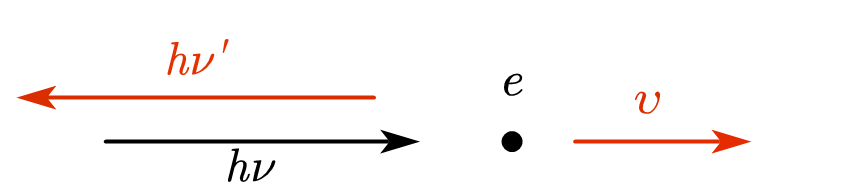
\includegraphics[width = 0.4\textwidth]{figure/康普顿散射正碰.png}
    \caption{康普顿散射正碰示意图}
\end{figure}
\begin{figure}[!h]
    \centering
    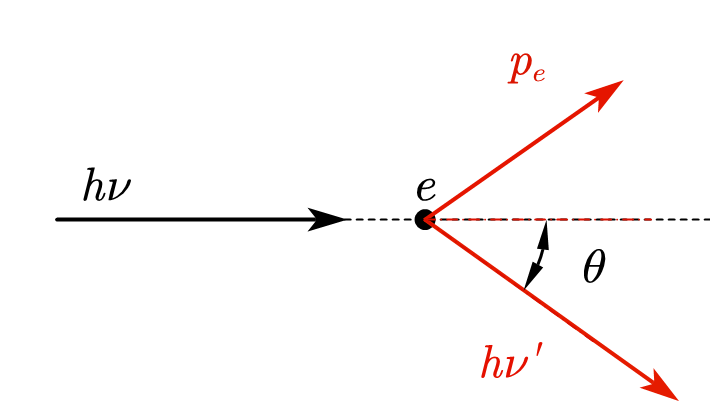
\includegraphics[width = 0.4\textwidth]{figure/康普顿散射示意图.png}
    \caption{康普顿散射示意图}
\end{figure}
\paragraph{Proof}
\begin{enumerate}
    \item $\displaystyle{when\  \theta = \pi,\lambda'-\lambda = \frac{2h}{m_ec}}$
    \item $\displaystyle{when\  \theta \neq \pi,\lambda'-\lambda = \frac{h}{m_ec}(1-\cos\theta)}$
\end{enumerate}
\paragraph{证明:}
\begin{enumerate}
    \item 设入射光子的动量为$\vec{p_i}$,能量为$E_i$,散射光子的动量为$\vec{p_f}$,能量为$E_f$,电子的动量为$p_e$,运动能量为$E_e$\\
          则有动量波长关系,以及相对论能量动量关系
          \begin{align*}
              p_i & = \frac{h}{\lambda}  & \quad E_i & = p_ic               \\
              p_f & = \frac{h}{\lambda'} & \quad E_f & = p_ec               \\
              ~   & ~                    & \quad E_e & = p_e^2c^2 +m_e^2c^4
          \end{align*}
          由动量守恒可知
          \begin{align*}
              \vec{p_i}             & = \vec{p_f}+\vec{p_e} \\
              \Rightarrow \vec{p_e} & = \vec{p_i}-\vec{p_e}
          \end{align*}
          两边同时平方,可得
          \begin{eqnarray*}
              p_e^2 = p_i^2+p_f^2-2p_ip_f\cos\theta
          \end{eqnarray*}
          由于此时的散射角$\theta = \pi$,因此有
          \begin{eqnarray*}
              p_e^2 = p_i^2+p_f^2+2p_ip_f
          \end{eqnarray*}
          由能量守恒可知
          \begin{eqnarray*}
              E_i+m_ec^2 = E_f +E_e\\
              \Rightarrow E_e = E_i-E_f+m_ec^2
          \end{eqnarray*}
          将其两边同时平方,可得
          \begin{eqnarray*}
              E_e^2 = (E_i-E_f+m_ec^2)^2
          \end{eqnarray*}
          利用上面给出的动量波长关系,以及相对论能量动量关系化简可得
          \begin{align*}
              \frac{1}{p_f}-\frac{1}{p_i}&=\displaystyle\frac{2}{m_ec}\\
              \Rightarrow \quad\lambda'-\lambda&=\displaystyle\frac{2h}{m_ec}
          \end{align*}




    \item 设入射光子的动量为$\vec{p_i}$,能量为$E_i$,散射光子的动量为$\vec{p_f}$,能量为$E_f$,电子的动量为$p_e$,运动能量为$E_e$\\
          则由第一问可知
          \begin{align*}
              p_e^2 = p_i^2+p_f^2-2p_ip_f\cos\theta \\
              E_e^2 = (E_i-E_f+m_ec^2)^2
          \end{align*}
          利用上面给出的动量波长关系,以及相对论能量动量关系化简可得
          \begin{eqnarray*}
              \frac{1}{p_f}-\frac{1}{p_i}=\frac{1}{m_ec}(1-\cos\theta)\\
              \Rightarrow \lambda'-\lambda=\frac{h}{m_ec}(1-\cos\theta)
          \end{eqnarray*}
\end{enumerate}

\section{算符与态矢}
\subsection{$\delta$函数的性质推导20240930}
Try to prove the properties of $\delta$ function:
\begin{enumerate}
    \item[(a)] $\displaystyle\delta(cx)=\frac{1}{|c|}\delta(x)$
    \item[(b)] $\displaystyle\delta(-x)=\delta(x)$
    \item[(c)] $\displaystyle\delta(g(x))=\sum_{i}\frac{\delta(x-x_i)}{|g'(x_i)|}\quad\quad where\ x=x_i\ is\ the\ root\ of\ function\ g(x)$
    \item[(d)] $\displaystyle\delta(x^2-a^2)=\frac{1}{2|a|}\left[\delta(x-a)+\delta(x+a)\right]$
    \item[(e)] $\displaystyle\int_{-\infty}^{+\infty}dx\delta(b-x)\delta(x-a)=\delta(a-b)$
\end{enumerate}



\begin{solution}
    

\begin{enumerate}
    \item[(a)] 根据Dirac一开始使用到的关于$\delta$函数的定义,我们可以得到
    \[\int_{-\infty}^{+\infty}dx\delta(x)=1\]
    于是我们有
    \begin{align*}
        \int_{-\infty}^{+\infty}dx\delta(cx)&=\frac{1}{c}\int_{-\infty}^{+\infty}d(cx)\delta(cx)\\
        &=1=\int_{-\infty}^{+\infty}dx\delta(x)
    \end{align*}
    将此处的$cx$看做是一个整体$t$,那么可以得到如下等式
    \[\int_{-\infty}^{+\infty}dt\frac{\delta(t)}{c}=\int_{-\infty}^{+\infty}dx\delta(cx)\]
    事实上,在这里$t$和$x$都只是一个记号,含义是一样的,因此,我们可以得到结论
    \[\delta(cx)=\frac{\delta(x)}{|c|}\]
    \item[(b)] 首先写出$\delta(x)$的定义
    \[\int_{-\infty}^{+\infty}dx\delta(x)=1\]
    代入$\delta(-x)$可以得到
    \begin{align*}
        \int_{-\infty}^{+\infty}dx\delta(-x)&=-\int_{-\infty}^{+\infty}d(-x)\delta(-x)\\
        &=\int_{+\infty}^{-\infty}d(-x)\delta(-x)\\
        &=1=\int_{-\infty}^{+\infty}d(t)\delta(t)
    \end{align*}
    因此有\[\delta(x)=\delta(-x)\]
    \item[(c)] 首先,对$g(x)$在其零点$x=x_i$处进行一节展开得到线性形式
    \begin{align*}
        g(x)=g(x_i)+g^{'}(x_i)(x-x_i)=g^{'}(x_i)(x-x_i)
    \end{align*}
    再根据$\delta$函数的定义,可以得到
    \begin{align*}
        \int dx\ \delta(g(x))&=\int dx\sum_{i}\delta(g^{'}(x_i)(x-x_i))\\
        &=\sum_{i}\frac{1}{|g^{'}(x)|}\int dx\ \delta(x-x_i)
    \end{align*}
    通过这个计算,可以得出
    \[
        \delta(g(x))=\sum_{i}\frac{\delta(x-x_i)}{|g^{'}(x_i)|}
    \]
    \item[(d)] 直接对这个$\delta$函数进行化简,可以得到
    \begin{align*}
        \delta(x^2-a^2)=\delta\left((x-a)(x+a)\right)
    \end{align*}
    可以观察到,这样的一个$\delta$函数,利用刚刚证明的性质,可以得到
    \begin{align*}
        \delta(x^2-a^2)&=\delta\left((x-a)(x+a)\right)\\
        &=\frac{\delta(x-a)}{|2a|}+\frac{x+a}{2|a|}\\
        &=\frac{1}{2|a|}\left[\delta(x-a)+\delta(x+a)\right]
    \end{align*}
    \item[(e)] 我们知道,对于$\delta $函数而言,有这样的作用
    \begin{align*}
        \int dx\delta(x-a)f(x)=f(a)
    \end{align*}
    这也就是说,$\delta(x-a)$可以将另外一个函数变成其在$x=a$处的取值,因此,证明这样的性质,我们也是一样,
    \begin{align*}
        \int dx \delta(b-x)\delta(x-a)=\int dx \delta(x-a)\delta(b-x)=\delta(b-a)
    \end{align*}
\end{enumerate}

\end{solution}







\subsection{简单的算符计算20240930}
Suppose two Operator $\hat{A},\hat{B}$ satisfy
\[\hat{A}^2=\hat{A}\hat{A}=0,\hat{A}\hat{A}^\dagger+\hat{A}^\dagger\hat{A}=1,B=\hat{A}\hat{A}^\dagger\]
\begin{enumerate}
    \item[(1)] Proof that $\hat{B}^2=\hat{B}$
    \item[(2)] Find out the matrix representation of $\hat{A},\hat{B}$
\end{enumerate}

\begin{solution}
    \ \\ \ 
    \begin{enumerate}
        \item[(1)] 下面开始证明,计算等式的左边
        \begin{align*}
            \hat{B}^2&=(\hat{A}\hat{A}^\dagger)(\hat{A}\hat{A}^\dagger)\\
            &=\hat{A}(1-\hat{A}\hat{A}^\dagger)\hat{A}^\dagger\\
            &=\hat{A}\hat{A}^\dagger-(\hat{A}\hat{A})(\hat{A}^\dagger\hat{A}^\dagger)\\
            &=\hat{A}\hat{A}^\dagger\\
            &=\hat{B}
        \end{align*}
        \item[(2)] 我们知道,算符$\hat{A}$满足$\hat{A}^2=0$的条件,为了简化我们的计算,我们考虑二维的希尔伯特空间,这样的话,我们可以得到
        \begin{align*}
            \hat{A}=\pmtwo{0}{1}{0}{0}
        \end{align*} 
        
        这时候验证一下我们的结论是否是正确的
        \begin{align*}
            \hat{A}\hat{A}^\dagger+\hat{A}^\dagger\hat{A}=\pmtwo{1}{0}{0}{1}
        \end{align*}
        
        很显然,这样求得的算符$\hat{A}$是满足条件的,那么自然而然的,通过这个,我么可以得出算符$B$的值
        \begin{align*}
            \hat{B}&=\hat{A}\hat{A}^\dagger\\
            &=\pmtwo{0}{1}{0}{0}\pmtwo{0}{0}{1}{0}\\
            &=\pmtwo{1}{0}{0}{0}
        \end{align*}
        
        于是,我们找到了一种满足条件的表示法。
    \end{enumerate}
\end{solution}





\subsection{本征值本征矢量的计算20240930}
\subsubsection{eigenvalues and eigenvectors}
Please find out the eigenvalues and eigenvectors of the following matrix and show the eigenvectors are orthogonal to each other.
\begin{enumerate}
    \item[(a)] \[\pmtwo{1}{2}{5}{4}\]
    \item[(b)] \[\pmtwo{-6}{3}{4}{5}\]
    \item[(c)] \[\pmtwo{0}{1}{-2}{3}\]
    \item[(d)] \[\pmtwo{0}{-2}{3}{4}\]
    \item[(e)] \[\pmtwo{-4}{-6}{3}{5}\]
    \item[(f)] \[\pmthree{2}{0}{0}{0}{4}{5}{0}{4}{3}\]
    \item[(g)] \[\pmthree{4}{6}{10}{3}{10}{13}{-2}{-6}{-8}\]
    \item[(h)] \[\pmthree{2}{2}{-2}{1}{3}{-1}{-1}{1}{1}\]
    \item[(i)] \[\pmthree{5}{-10}{-5}{2}{14}{2}{-4}{-8}{6}\]
\end{enumerate}


\begin{solution}
\begin{enumerate}
    \item[a] 该矩阵的本征行列式为$\vmtwo{1-\lambda}{2}{5}{4-\lambda}$
    
    令其本征行列式值为零求解其本征值
    \begin{align*}
        \vmtwo{1-\lambda}{2}{5}{4-\lambda}&=0\\
        (\lambda-6)(\lambda+1)&=0
    \end{align*}
    因此本征值$\lambda=6,-1$,将其分别带入到方程当中,我们可以得到两个本征矢量。
    \[\begin{pmatrix}
        2\\
        5
    \end{pmatrix}和
    \begin{pmatrix}
        -1\\
        1
    \end{pmatrix}\]
    通过施密特正交化过程,我们可以得到两个正交归一的本征矢量
    \[\begin{pmatrix}
        \frac{1}{\sqrt{2}}\\
        \frac{1}{\sqrt{2}}
    \end{pmatrix}和
    \begin{pmatrix}
        -\frac{1}{\sqrt{2}}\\
        \frac{1}{\sqrt{2}}
    \end{pmatrix}\]
    \item[b] 该矩阵的本征行列式为$\vmtwo{-6-\lambda}{3}{4}{5-\lambda}$
    
    令其本征行列式值为零求解其本征值
    \begin{align*}
        \vmtwo{-6-\lambda}{3}{4}{5-\lambda}&=0\\
        (\lambda-6)(\lambda+7)&=0
    \end{align*}
    因此本征值$\lambda=6,-7$,将其分别带入到方程当中,我们可以得到两个本征矢量。
    \[\begin{pmatrix}
        1\\
        4
    \end{pmatrix}和
    \begin{pmatrix}
        -3\\
        1
    \end{pmatrix}\]
    通过施密特正交化过程,我们可以得到两个正交归一的本征矢量
    \[\begin{pmatrix}
        \frac{3}{\sqrt{10}} \\ 
        -\frac{1}{\sqrt{10}} \\
    \end{pmatrix}和
    \begin{pmatrix}
        \frac{1}{\sqrt{10}} \\
        \frac{3}{\sqrt{10}} 
    \end{pmatrix}\]
    \item[c] 该矩阵的本征行列式为$\vmtwo{-\lambda}{1}{-2}{3-\lambda}$
    
    令其本征行列式值为零求解其本征值
    \begin{align*}
        \vmtwo{-\lambda}{1}{-2}{3-\lambda}&=0\\
        (\lambda-2)(\lambda-1)&=0
    \end{align*}
    因此本征值$\lambda=2,1$,将其分别带入到方程当中,我们可以得到两个本征矢量。
    \[\begin{pmatrix}
        1\\
        2
    \end{pmatrix}和
    \begin{pmatrix}
        1\\
        1
    \end{pmatrix}\]
    通过施密特正交化过程,我们可以得到两个正交归一的本征矢量
    \[\begin{pmatrix}
        \frac{1}{\sqrt{2}}\\
        \frac{1}{\sqrt{2}}
    \end{pmatrix}和
    \begin{pmatrix}
        -\frac{1}{\sqrt{2}}\\
        \frac{1}{\sqrt{2}}
    \end{pmatrix}\]
    \item[d]
\end{enumerate}
\end{solution}






\subsubsection{Complex and Rotation Matrix}
\begin{enumerate}
    \item Find out eigenvalues and eigenvectors of following complex matrix.
    \[A=\pmthree{2}{0}{-2}{-2i}{i}{2i}{1}{0}{-1}\]
    \item The $2\times 2$rotation matrix in $x-y$ plane can be written as
    \[R=\pmtwo{\cos\theta}{-\sin\theta}{\sin\theta}{\cos\theta}\]
    Show that rotation matrix do not have real eigenvalues and find the complex eigenvalues and eigenvectors.
\end{enumerate}






\subsection{对易的性质20241010}
Theorem of simultanoues diagonaligability.Let $\hat{A},\hat{B}\in M_n(\mathbb{C})$,the set of all $n\times n$ matrics with complex entries,be diagonaligable. Then $[A,B]=0$, if and only there is an invertible $S\in M_n(\mathbb{C})$ ,such that $SAS^{-1} \ and\  SBS^{-1}$ are both diagonal.

\begin{solution}
    假设$[A,B] =0$,即$AB=BA$。由于A和B都是可对角化的矩阵,所以我们可以找到与A和B对角化的矩阵。

    由于$A$是可对角化的,因此存在一个可逆矩阵$P$使得$P^{-1}AP$是对角矩阵,记作$A'$。接下来考虑B在坐标变化$P$下的表示,即$B^\prime=P^{-1}BP$。由于$AB=BA$,因此我们将会有:
    \begin{align*}
        A'B'=P^{-1}APP^{-1}BP&=P^{-1}ABP\\
        &=P^{-1}BAP\\
        &=B'A'
    \end{align*}

    由此可见,$[A',B']=0$

    又由于$A'$是对角矩阵,这意味着$𝐵′$可以写成块对角矩阵的形式,其中每个块与$A$的特征值对应的特征空间相匹配。于是我们得到了$B$也可对角化的性质,因此在相似变化$P^{-1}BP$下$B'$也可以被对角化。这个时候,我们给定一个可逆矩阵$Q$,并令$S=PQ$,使得$SBS^{-1}$是一个对角阵。

    下面来进行验证一下
    \begin{align*}
        SAS^{-1}&=PQAQ^{-1}P^{-1}=(Q^{-1}P^{-1}APQ)^*=Q^{-1}diag(\lambda_A)Q=diag(\lambda_A)\\
        SBS^{-1}&=PQBQ^{-1}P^{-1}=diag(\lambda_B)
    \end{align*}
此时,𝑆𝐴𝑆−1 和𝑆𝐵𝑆−1 都是对角矩阵。
\end{solution}

\section{一维定态薛定谔方程}
\subsection{不确定性关系20241011}
\paragraph{Proof}that $[E,t]=i\hbar$ and thus $\displaystyle\Delta_\psi E\Delta_\psi t\geqslant \frac{\hbar}{2}$


\begin{proof}
    由薛定谔方程我们可以有
    \begin{align*}
        E\psi(t)=i\hbar\frac{\partial}{\partial t}\psi(t)
    \end{align*}

    因此,我们可以有对应关系
    \[E=i\hbar\frac{\partial}{\partial t}\]

    下面我们将其作用到态函数上来求解其对易关系$[E,t]$所对应的本征值
    \begin{align*}
        [E,t]\psi(t)&=(Et-tE)\psi(t)\\
        &=i\hbar\frac{\partial}{\partial t}\left(t\psi(t)\right)-i\hbar t\frac{\partial}{\partial t}\psi(t)\\
        &=i\hbar\left(\psi(t)+t\frac{\partial}{\partial t}\psi(t)\right)-i\hbar t\frac{\partial}{\partial t}\psi(t)\\
        &=i\hbar\psi(t)
    \end{align*}
    
    由此可见,$[E,t]$所对应的本征值为$i\hbar$
    
    因此,\[[E,t]=i\hbar\]

    接下来需要证明的就是不确定性关系,这一段直接抄笔记。

    定义$\expectation{A}_\psi=\bek{\psi}{A}{\psi},\ket{\psi_A}=\expectation{A-\expectation{A}}_{\psi}\ket{\psi},$且$\braket{\psi}{\psi}=1$

    因此我们可以有
    \begin{align*}
        \braket{\psi_A}{\psi_A}&=\bek{\psi}{\left(A-\expectation{A}_\psi\right)^2}{\psi}\\
        &=\bek{\psi}{\left(A^2-2A\expectation{A}_\psi+\expectation{A}_\psi^2\right)}{\psi}\\
        &=\expectation{A^2}_\psi-\expectation{A}_\psi^2\\
        &=\sigma_A^2
    \end{align*}

    由Cauchy-Schwarz不等式,我们可以有
    \begin{align*}
        \left|\braket{\psi_A}{\psi_B}\right|^2&\leq \braket{\psi_A}{\psi_A}\braket{\psi_B}{\psi_B}=\sigma_A^2\sigma_B^2
    \end{align*}

    于是我们便可以知道
    \begin{align*}
        \braket{\psi_A}{\psi_B}&=\bek{\psi}{\left(A-\expectation{A}_\psi\right)\left(B-\expectation{B}_\psi\right)}{\psi}\\
        &=\bek{\psi}{AB-A\expectation{B}_\psi-\expectation{A}_\psi B+\expectation{A}_\psi\expectation{B}_\psi}{\psi}\\
        &=\expectation{AB}_\psi-\expectation{A}_\psi\expectation{B}_\psi
    \end{align*}
\end{proof}








\subsection{一维无限势阱20241011}
Consider an 1-D infinite wall for
\[
        V(x)=\begin{cases}
                0&,\quad -\frac{L}{2}<  x<\frac{L}{2} \\
                \infty&,\quad |x|>\frac{L}{2}
            \end{cases}
\]
\begin{enumerate}
    \item work out the wave function and energy spectrum.
    \item Proof that 
    \begin{equation*}
        \int dx \phi_n^{*}(x)\phi_m(x)=\delta_{nm}
    \end{equation*}
    \item Caculate the expectation value of $\expectation{x},\expectation{x^2},\expectation{p},\expectation{p^2}$ for $\phi_1,\phi_2,\phi_3$,and check the uncertainly principle.
    \item Try to plot the wave function $\phi_n(x)$for $n=1,2,3$
\end{enumerate}

\begin{figure}[hbtp]
    \centering
    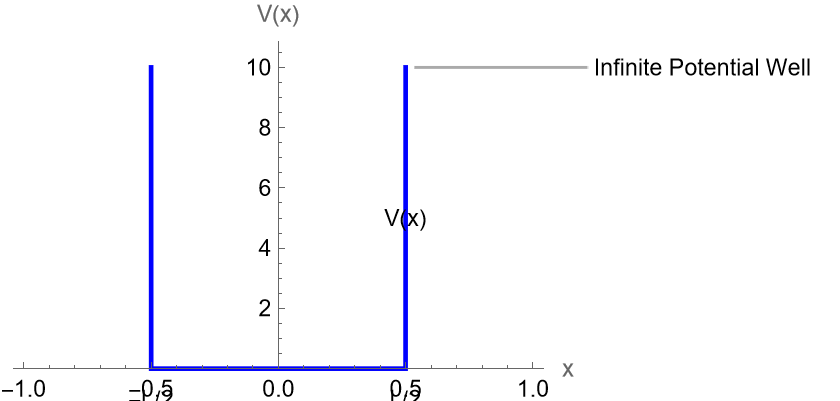
\includegraphics[width=0.8\textwidth]{figure/一维无线深方势阱.png}
    \caption{一维无限深方势阱}
    \label{fig:一维无限势阱}
\end{figure}


\begin{solution}
    \begin{enumerate}
        \item[(1)] 很显然,在势阱的内部势能为$0$,因此我们可以将定态薛定谔方程写为
    \begin{equation*}
        \frac{d^2}{dx^2}\psi=k^2\psi,\quad k^2=-\frac{2mE}{\hbar^2}
    \end{equation*}
    我们可以得到通解
    \begin{equation*}
        \psi(x)=A\sin{kx}+B\cos{kx}
    \end{equation*}
    这个问题的波函数是在势阱当中,而波函数是不能够自由的存在于一个势垒里面的,它应该很快就会弥散掉,这也就意味着在边界处,波函数的值应当为$0$,因此我们得到了第一个边界条件
    \begin{align*}
        &\psi(-\frac{L}{2})=\psi(\frac{L}{2})=0\\
        \Rightarrow&
        \begin{cases}
            A\sin{\frac{L}{2}k}+B\cos{\frac{L}{2}k}=0\\
            -A\sin{\frac{L}{2}k}+B\cos{\frac{L}{2}k}=0
        \end{cases}
    \end{align*}
    但是仅仅凭借这个条件,我们并不能够确定$A,B$到底哪一个应该为$0$

    容易想到,波函数一定是关于$x=0$处对称的(这里并不一定,我犯了一个错误,事实上也是可以反对称的也就是中心对称,这里的假设导致我最后得到的是一个偶函数解),所以可以很自然的想到,$x=0$应当是一个极值点,因此我们可以有
    \begin{align*}
        \left.\D{\psi}{x}\right|_{x=0}&=0\\
        \Rightarrow\left.\left[A\cos{kx}-B\sin{kx}\right]\right|_{x=0}&=0\\
        \Rightarrow A&=0
    \end{align*}
    于是我们便可以知道
    \begin{equation*}
        \psi(x)=B\cos{kx}
    \end{equation*}
    将其带入到第一个边界条件当中,可以得到
    \begin{equation*}
        k_n=\frac{(2n-1)\pi}{L}
    \end{equation*}
    由此,波函数可以写为
    \begin{equation*}
        \psi_n(x)=B\cos{\frac{(2n-1)\pi}{L}x}
    \end{equation*}
    至此,剩余一个未知量$B$,利用归一化条件,可以得出
    \begin{align*}
        B_n^2\int_{-\frac{L}{2}}^{\frac{L}{2}}\cos^2{\frac{(2n-1)\pi}{L}x}\ dx&=1\\
        2k&=kLB_n^2\\
        B_n&=\sqrt{\frac{2}{L}}
    \end{align*}
    于是我们找到了对应的波函数
    \begin{align*}
        \psi_n(x)=\sqrt{\frac{2}{L}}\cos{\frac{(2n-1)\pi}{L}x}
    \end{align*}

    接下来开始求解奇函数解这也就是说,我们直接令$B=0$,得到
    \begin{align*}
        \psi(x)=A\sin{kx}
    \end{align*}
    将其代入到第一个边界条件当中,可以得到
    \begin{align*}
        k_n=\frac{2n\pi}{L}
    \end{align*}

    得到波函数表达式为
    \begin{align*}
        \psi_n(x)=A_n\sin{\frac{2n\pi}{L}x}
    \end{align*}

    进行归一化,得到波函数表达式为
    \begin{align*}
        \psi_n(x)=\sqrt{\frac{2}{L}}\sin{\frac{2n\pi}{L}x}
    \end{align*}
    \item[(2)] 问题二要求我们去证明波函数的正交性,我们可以通过计算
    \begin{align*}
        \int dx \phi_n^{*}(x)\phi_m(x)=\int dx \psi_n(x)\psi_m(x)
    \end{align*}

    那么就近计算一下
    其中,归一化后的波函数为: 
    \[ 
        \psi_n(x) = \sqrt{\frac{2}{L}} \sin\left(\frac{2n\pi}{L} x\right) 
    \] 
    对于不同的量子数 $ m $ 和 $ n $,我们需要计算以下积分: 
    \[ 
        \int_{-\frac{L}{2}}^{\frac{L}{2}} \sin\left(\frac{2m\pi}{L} x\right) \sin\left(\frac{2n\pi}{L} x\right) \, dx 
    \] 
    
    利用正交函数的性质,我们可以推导出以下结果: 
    \begin{enumerate}
        \item 当 $ m = n $ 时: 
        \[ 
            \int_{-\frac{L}{2}}^{\frac{L}{2}} \sin^2\left(\frac{2n\pi}{L} x\right) \, dx = \frac{L}{2}
         \]
        \item 当 $ m \ne n $ 时: 
        \[ 
            \int_{-\frac{L}{2}}^{\frac{L}{2}} \sin\left(\frac{2m\pi}{L} x\right) \sin\left(\frac{2n\pi}{L} x\right) \, dx = 0 
        \] 
    \end{enumerate}
    
    接下来开始证明,经过计算可以得到
    \begin{align*}
        &\int_{-\frac{L}{2}}^{\frac{L}{2}} \sin\left(\frac{2m\pi}{L} x\right) \sin\left(\frac{2n\pi}{L} x\right)\\
        &=\frac{L n \sin (\pi  m) \cos (\pi  n)-L m \cos (\pi  m) \sin (\pi  n)}{\pi  \left(m^2-n^2\right)}\\
        &=\frac{L m \sin (\pi  m-\pi  n)+L n \sin (\pi  m-\pi  n)-L m \sin (\pi  m+\pi  n)+L n \sin (\pi  m+\pi  n)}{2 \pi  \left(m^2-n^2\right)}
    \end{align*}
    这样,让$m=n$,就可以很容易得到
    \begin{align*}
        \int_{-\frac{L}{2}}^{\frac{L}{2}} \sin^2\left(\frac{2n\pi}{L} x\right) \, dx = \frac{L}{2}
    \end{align*}
    
    让$m\neq n$,可以得到
    \[ 
            \int_{-\frac{L}{2}}^{\frac{L}{2}} \sin\left(\frac{2m\pi}{L} x\right) \sin\left(\frac{2n\pi}{L} x\right) \, dx = 0 
    \] 
    综上,我们证明了
    \begin{equation*}
        \int dx \phi_n^{*}(x)\phi_m(x)=\delta_{nm}
    \end{equation*}

    \item[(3)] 接下来计算一下前三个波函数$\phi_1,\phi_2,\phi_3$所对应的$\expectation{x},\expectation{x^2},\expectation{p},\expectation{p^2}$
    先给出我们的波函数的通解
    \begin{align*}
        \psi_n(x)=\sqrt{\frac{2}{L}}\sin{\frac{2n\pi}{L}x}
    \end{align*}
    接下来我们来计算一下对于$\phi_n$而言的$\expectation{x},\expectation{x^2},\expectation{p},\expectation{p^2}$

    首先是$\expectation{x}$
    \begin{align*}
        \expectation{x}&=\int_{-\frac{L}{2}}^{\frac{L}{2}}\ x\left(\sqrt{\frac{2}{L}}\sin{\frac{2n\pi}{L}x}\right)^2\ dx\\
    \end{align*}
    很显然,这个函数是一个奇函数,因此对于对称区间上的积分应该是为$0$的,所以我们有
    \begin{align*}
        \expectation{x}=0
    \end{align*}

    接着是$\expectation{x^2}$,直接偷个懒,使用mma计算得出
    \begin{align*}
        \expectation{x^2}&=\int_{-\frac{L}{2}}^{\frac{L}{2}}\ x^2\left(\sqrt{\frac{2}{L}}\sin{\frac{2n\pi}{L}x}\right)^2\ dx\\
        &=\frac{L^2}{12}\left(1-\frac{1}{4n^2\pi^2}\right)
    \end{align*}

    然后是$\expectation{p}$
    \begin{align*}
        \expectation{p}&=\int_{-\frac{L}{2}}^{\frac{L}{2}}\ i\hbar\frac{d}{dx}\left(\sqrt{\frac{2}{L}}\sin{\frac{2n\pi}{L}x}\right)^2\ dx\\
    \end{align*}
    对于这样的一个积分,是对一个偶函数进行求导,那么得到的应当是一个奇函数,所以这个的积分值仍然为$0$,即
    \begin{align*}
        \expectation{p}=0
    \end{align*}

    最后,就是计算我们的$\expectation{p^2}$,继续使用mma
    \begin{align*}
        \expectation{p^2}&=-\hbar^2\int_{-\frac{L}{2}}^{\frac{L}{2}}\ \frac{d^2}{dx^2}\left(\sqrt{\frac{2}{L}}\sin{\frac{2n\pi}{L}x}\right)^2\ dx\\
        &=\frac{4\hbar^2n^2\pi^2}{L^2}
    \end{align*}

    验证一下测不准原理
    \begin{align*}
        \Delta x\Delta p&=\sqrt{\left(\expectation{x^2}-\expectation{x}^2\right)\left(\expectation{p^2}-\expectation{p}^2\right)}\\
        &=\sqrt{\frac{1}{12}\left(1-\frac{1}{4n^2\pi^2}\right)}\cdot 2\hbar n\pi\geqslant\frac{\hbar}{2}
    \end{align*}
    下面就是代入到$n=1,2,3$的波函数当中了
    \begin{enumerate}
        \item[n=1] 
        \begin{align*}
            \phi_1(x)&=\sqrt{\frac{2}{L}}\sin{\frac{2\pi x}{L}}\\
            \expectation{x}&=0\\
            \expectation{x^2}&=\frac{L^2}{12}\left(1-\frac{1}{4\pi^2}\right)\\
            \expectation{p}&=0\\
            \expectation{p^2}&=\frac{4\hbar^2\pi^2}{L^2}
        \end{align*}
        
        \item[n=2] 
        \begin{align*}
            \phi_1(x)&=\sqrt{\frac{2}{L}}\sin{\frac{4\pi x}{L}}\\
            \expectation{x}&=0\\
            \expectation{x^2}&=\frac{L^2}{12}\left(1-\frac{1}{16\pi^2}\right)\\
            \expectation{p}&=0\\
            \expectation{p^2}&=\frac{16\hbar^2\pi^2}{L^2}
        \end{align*}
        \item[n=3]
        \begin{align*}
            \phi_1(x)&=\sqrt{\frac{2}{L}}\sin{\frac{8\pi x}{L}}\\
            \expectation{x}&=0\\
            \expectation{x^2}&=\frac{L^2}{12}\left(1-\frac{1}{36\pi^2}\right)\\
            \expectation{p}&=0\\
            \expectation{p^2}&=\frac{36\hbar^2\pi^2}{L^2}
        \end{align*}
    \end{enumerate}
    \item[(4)] 接下来,我将给出$\phi_1,\phi_2,\phi_3$在势阱中的的图像 
    \begin{figure}[hbtp]
        \centering
        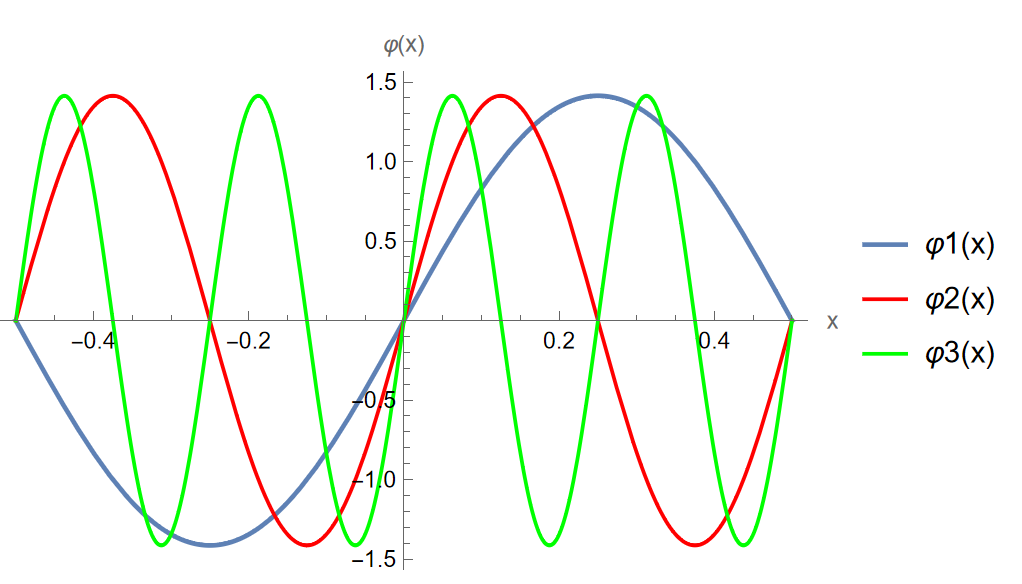
\includegraphics[width=0.5\textwidth]{figure/一维无线深方势阱的波函数解.png}
        \caption{The wave function of the first three states in the potential well}
        \label{fig:wave_function}
    \end{figure}
    \end{enumerate}
    
        
\end{solution}


\subsection{Hamitionian Oscillator-1 20241014}
One of the expression of the Hermite polynomials is
\begin{equation*}
    H_n(x)=(-1)^ne^{y^2}\left(\frac{d}{dy}\right)^ne^{-y^{2}}
\end{equation*}
\begin{enumerate}
    \item[(1)] Derive the expression of $H_0,H_1,\cdots,H_4$
    \item[(2)] The differential equation of the Hermite polynomials is
    \begin{equation*}
        H_n^{''}(y)-2yH_n^{'}(y)+2nH_n(y)=0
    \end{equation*}
    it can be written as
    \begin{equation*}
        H_{n+1}(y)=2yH_n(y)-2nH_{n-1}(y)
    \end{equation*}
    By using
    \begin{equation*}
        \frac{\partial H_n(y)}{\partial y}=2nH_n(y)
    \end{equation*}
    Please derive $H_5,H_6$.
    \item[(3)] Sketch $H_0,H_1,\cdots,H_6$.
    \item[(4)] By using normalization condition,try to find out 
    \begin{equation*}
        \psi_n(x)=\left(\frac{m\omega}{\pi\hbar}\right)^{\frac{1}{4}}\frac{1}{\sqrt{2^nn!}}H_n(y)e^{-y^2}
    \end{equation*}
    \item[(5)] Please verify the orthogonal condition
    \begin{equation*}
        \int dx\ \psi_n^{*}(x)\psi_m(x)=\delta_{nm}
    \end{equation*}
\end{enumerate}


\begin{solution}
    \begin{enumerate}
        \item[(1)] 通过使用厄米多项式给出的计算公式,我们可以进行如下的计算
        \begin{align*}
            H_0(y)&=e^{y^2}e^{-y^2}=1\\
            H_1(y)&=(-1)^1e^{y^2}\frac{d}{dy}e^{-y^2}\\
            &=-e^{y^2}(-2ye^{-y^2})=2y\\
            H_2(y)&=(-1)^2e^{y^2}\frac{d}{dy}\left(-2ye^{-y^2}\right)\\
            &=4y^2-2\\
            H_3(y)&=(-1)^3e^{y^2}\frac{d}{dy}\left(e^{-y^2}(4y^2-2)\right)\\
            &=8y^3-12y\\
            H_4(y)&=(-1)^4e^{y^2}\frac{d}{dy}\left(e^{-y^2}(8y^3-12y)\right)\\
            &=16y^4-48y^2+12
        \end{align*}
        值得一提的是,在这里,我们已经可以发现公式$\displaystyle H_n(y)=(-1)^n e^{y^2}\left(\frac{d}{dy}\right)^n e^{-y^2}$再求导的时候,其实就是再对$e^{-y^2}H_{n-1}(y)$进行一个求导
        \item[(2)] 仍然是利用题目当中所给到的公式进行一个计算,需要计算的是$H_5,H_6$
        \begin{align*}
            H_5(y)&=2yH_4(y)-2*4H_3(y)\\
            &=32y^5-160y^3+120y\\
            H_6(y)&=2yH_5(y)-2*5H_4(y)\\
            &=64y^6-480y^4+720y^2-120
        \end{align*}
        \item[(3)] 给出我是用mma画出来的$H_0,H_1,\cdots H_6$的图像
        \begin{figure}[hbtp]
            \centering
            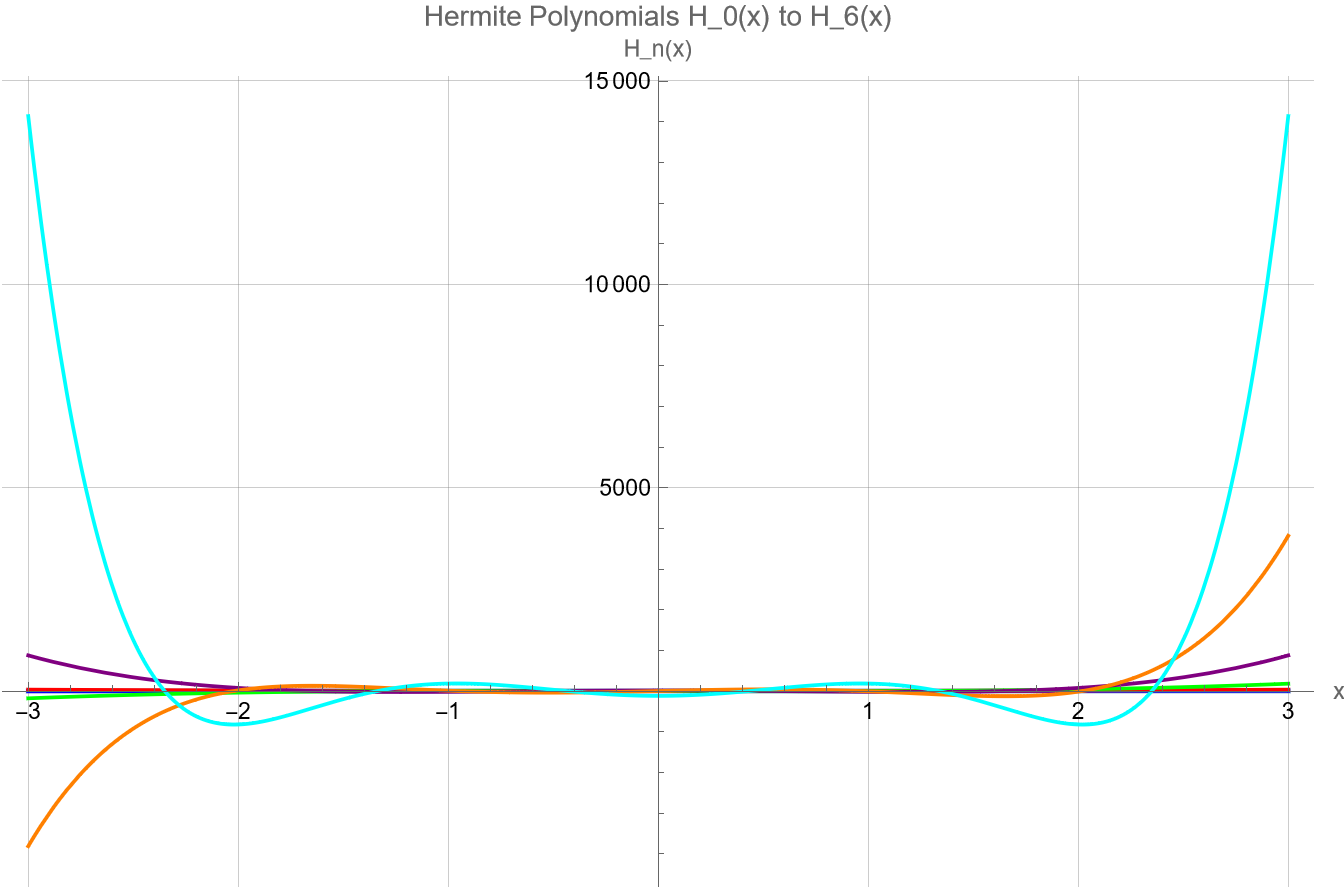
\includegraphics[width=0.5\textwidth]{figure/厄米多项式.png}
            \caption{$H_0,H_1,\cdots H_6$的图像}
        \end{figure}
        
        这个图中几乎已经看不到前几项厄米多项式了,而$H_6$的图像可以看得很清晰,这也就是说,厄米多项式在之后将会增长得非常快,挺让人担忧波函数会不会爆掉。
        \item[(4)] 要求我们使用归一化的条件来求出波函数$\psi_n(x)$的表达式
        
        简谐振子的波函数可以表示为
        \begin{align*}
            \psi_n(x)&=N_nH_n\left(\sqrt{\frac{m\omega}{\hbar}}x\right)e^{-\frac{m\omega x^2}{2\hbar}}
        \end{align*}
        有归一化条件,我们可以有
        \begin{align*}
            \int dx\ \psi_n^{*}(x)\psi_n(x)&=1
        \end{align*}
        现在,为了计算的方便,令$\displaystyle y=\sqrt{\frac{m\omega}{\hbar}}x$,则$\displaystyle dx=\sqrt{\frac{\hbar}{m\omega}}dy$

        则有
        \begin{align*}
            \int_{-\infty}^{\infty}|N_n|^2|H_n(y)|^2e^{-y^2}\sqrt{\frac{\hbar}{m\omega}}dy&=1\\
            |N_n|^2\sqrt{\frac{\hbar}{m\omega}}\int_{-\infty}^{\infty}|H_n(y)|^2e^{-y^2}dy&=1
        \end{align*}
        对于这样的复杂式子,我是一点耐心都没有,直接上mma吧,最终我们可以得到
        \begin{align*}
            N_n=\left(\frac{m\omega}{\pi\hbar}\right)^{\frac{1}{4}}\frac{1}{\sqrt{2^nn!}}
        \end{align*}
        OK!这样我们就成功的归一化了。

        \item[(5)] 这一小问是要我们证明一下这个波函数的正交性,还是和之前一样的操作,任意取两个波函数$\psi_n,\psi_m$
        \begin{align*}
            \psi_n(x)&=N_nH_n\left(\sqrt{\frac{m\omega}{\hbar}}x\right)e^{-\frac{m\omega x^2}{2\hbar}}\\
            \psi_m(x)&=N_mH_m\left(\sqrt{\frac{m\omega}{\hbar}}x\right)e^{-\frac{m\omega x^2}{2\hbar}}
        \end{align*}

        接下来就是要计算积分$\displaystyle\int dx\ \psi_n^{*}(x)\psi_m(x)$了,还是一样,直接使用mma
        \begin{align*}
            \int dx\ \psi_n^{*}(x)\psi_m(x)&=\left(\frac{m\omega}{\pi\hbar}\right)^{\frac{1}{2}}\sqrt{\frac{\hbar}{m\omega}}\sqrt{\pi}\delta_{nm}\\
            &=\delta_{nm}
        \end{align*}
    \end{enumerate}
\end{solution}















\subsection{Hamitionian Oscillator-2 20241014}
By using 
\begin{align*}
    (a_{+}a_{-}+\frac{1}{2}\hbar\omega)\psi(x)&=E\psi(x)\\
    (a_{+}a_{-}-\frac{1}{2}\hbar\omega)\psi(x)&=E\psi(x)
\end{align*}

And normalization condition
\begin{equation*}
    \int dx\ \psi_n^{*}(x)\psi_n(x)=1,\quad for\ all\ n
\end{equation*}

\begin{enumerate}
    \item[(a)] Show that 
    \begin{align*}
        \int dx |a_{+}\psi_n(x)|^2&=(n+1)\hbar\omega\\
        \int dx |a_{-}\psi_n(x)|^2&=n\hbar\omega
    \end{align*}
    and thus 
    \begin{align*}
        a_{+}\ket{\psi_n(x)}&=\sqrt{(n+1)\hbar\omega}\ket{\psi_{n+1}(x)}\\
        a_{-}\ket{\psi_n(x)}&=\sqrt{n\hbar\omega}\ket{\psi_{n-1}(x)}
    \end{align*}
    \item[(b)] By using the result of (a),determine the normalization factor of $\ket{\psi_n(x)}$:
    \begin{align*}
        \psi_n(x)&=C(a_+)^ne^{-\frac{m\omega}{2\hbar}x^2}\\
        C&=\left(\frac{m\omega}{\pi\hbar}\right)^{\frac{1}{4}}\frac{(-1)^n}{n!(\hbar\omega)^n}
    \end{align*}
\end{enumerate}

\begin{solution}
    \begin{enumerate}
        \item[(a)] 我们知道
        \begin{align*}
            H\psi_n(x)&=\left(a_+a_-+\frac{1}{2}\hbar\omega\right)\psi_n(x)=E_n\psi_n(x)\\
            H\psi_n(x)&=\left(a_-a_+-\frac{1}{2}\hbar\omega\right)\psi_n(x)=E_n\psi_n(x)\\
            E_n&=\left(n+\frac{1}{2}\right)\hbar\omega
        \end{align*}

        因此,我么可以得到
        \begin{align*}
            \left(a_+a_-+\frac{1}{2}\hbar\omega\right)\psi_n(x)&=\left(n+\frac{1}{2}\right)\hbar\omega\psi_n(x)\\
           \left(a_-a_+-\frac{1}{2}\hbar\omega\right)\psi_n(x)&=\left(n+\frac{1}{2}\right)\hbar\omega\psi_n(x)
        \end{align*}

        这也就是说
        \begin{align*}
            a_+a_-\psi_n(x)&=n\hbar\omega\psi_n(x)\\
            a_-a_+\psi_n(x)&=\left(n+1\right)\hbar\omega\psi_n(x)
        \end{align*}

        于是

$$\begin{aligned}
\int|a_{+}\psi_{n}(x)|^{2}dx& =\int(a_{+}\psi_{n}(x))^{*}(a_{+}\psi_{n}(x))dx  \\
&=\int(a_{-}\psi_{n}^{*}(x))(a_{+}\psi_{n}(x))dx \\
&=(n+1)\hbar\omega 
\end{aligned}$$

$$\begin{aligned}
\int|a_{-}\psi_{n}(x)|^{2}dx& =\int(a_{-}\psi_{n}(x))^{*}(a_{-}\psi_{n}(x))dx  \\
&=\int(a_{+}\psi_{n}^{*}(x))(a_{-}\psi_{n}(x))dx \\
&=n\hbar\omega 
\end{aligned}$$

由于

$$a_-a_+-a_+a_-=\hbar\omega $$

故

$$a_-a_+|\psi_n\rangle=(a+a-+\hbar w)|\psi_n\rangle $$

令$a_{+ }| \psi _{n}\rangle = C_{n}| \psi _{n+ 1}\rangle$ , $a_{- }| \psi _{n}\rangle = D_{n}| \psi _{n- 1}\rangle$

$$H=a_-a_+-\frac{1}{2}\hbar w$$

$$H|\psi_n\rangle=E|\psi_n\rangle $$

$$(a_-a_+-\frac{1}{2}\hbar\omega)|\psi_n\rangle=(n+\frac{1}{2})\hbar\omega|\psi_n\rangle $$

$$a_-a_+|\psi_n\rangle=(n+1)\hbar w|\psi_n\rangle $$

同理可得

$$a_+a_-|\psi_n\rangle=n\hbar w|\psi_n\rangle $$

由于

$$\langle\psi_n|a_-a_+|\psi_n\rangle=(n+1)\hbar\omega\langle\psi_n|\psi_n\rangle $$
\item[(b)]
对$\psi_{0}(x)=Ae^{-\frac{m\omega x^{2}}{2h}}$ 进行归一化处理可得

$$\begin{aligned}
\int_{-\infty}^{\infty}|\psi_{0}(x)|^{2}dx& =1 \\
A^{2}\int_{-\infty}^{\infty}e^{-{\frac{m\omega x^{2}}{h}}}dx& =1 \\
A^{2}\:\sqrt{\frac{\pi\hbar}{m\omega}}& =1 
\end{aligned}$$

得到

$$A=\left(\frac{m\omega}{\pi\hbar}\right)^{\frac{1}{4}}$$

综上所述

$$C=\left(\frac{m\omega}{\pi\hbar}\right)^{\frac{1}{4}}\frac{(-1)^n}{\sqrt{n!(\hbar\omega)^n}}$$
        
    \end{enumerate}
\end{solution}

























\subsection{Hamitionian Oscillator in 3-D 20241014}
Consider harmonic oscillator in 3-D. The Hamiltonian is
\begin{equation*}
    H=-\frac{\hbar^2}{2m}\left(\frac{\partial^2}{\partial x_1^2}+\frac{\partial^2}{\partial x_2^2}+\frac{\partial^2}{\partial x_3^2}\right)+\frac{1}{2}m\omega^2\left(x_1^2+x_2^2+x_3^2\right)
\end{equation*}

\begin{enumerate}
    \item[(1)] Try to find out the wave function and energy of ground state by using
    \begin{equation*}
        a_{i\pm }=\frac{1}{\sqrt{2m}}\left(\frac{\hbar}{i}\Da{~}{x_i}\mp im\omega x_i\right),\quad i=1,2,3
    \end{equation*}
    \item[(2)] Work out $[a_{i-},a_{j+}],[a_{i-},a_{j-}],[a_{i+},a_{j-}]$
\end{enumerate}

\subsection{对易关系的常见性质(补)20241021}

Try to verify
\begin{enumerate}
    \item $\left[A+B,C\right]=\left[A,C\right]+\left[B,C\right]$
    \item $\left[A,\left[B,C\right]\right]+\left[B,\left[C,A\right]\right]+\left[C,\left[A,B\right]\right]=0$
    \item $[A,BC]=[A,B]C+B[A,C]$
    \item $[AB,C]=A[B,C]+[A,C]B$
    \item $[A,BCD]=[A,B]CD+B[A,C]D+BC[A,D]$
    \item $[ABC,D]=AB[C,D]+A[B,D]C+[A,D]BC$
\end{enumerate}

\begin{solution}
    \begin{enumerate}
        \item 
        \begin{align*}
            [A+B,C]&=(A+B)C-C(A+B)\\
            &=AC+BC-CA-CB\\
            &=[A,C]+[B,C]
            \end{align*}
        \item 
        \begin{align*}
            [A,[B,C]]+[B,[C,A]]+[C,[A,B]]&=A[B,C]+[B,C]A+B[C,A]+[C,A]B+C[A,B]+[A,B]C\\
            &=ABC-ACB+BCA-CBA+BCA-CBA\\
            &+CAB-ACB+ABC-BAC\\
            &=0
        \end{align*}
        \item 
        \begin{align*}
            [A,BC]&=ABC-BCA\\
            &=ABC-BAC+BAC-BCA\\
            &=[A,B]C+B[A,C]    
        \end{align*}
        \item 
        \begin{align*}
            [AB,C]&=ABC-CAB\\
            &=ABC-ACB+ACB-CAB\\
            &=A[B,C]+[A,C]B    
        \end{align*}
        \item 
        \begin{align*}
            [A,BCD]&=ABCD-BCDA\\
            &=ABCD-BACD+BACD-BCAD+BCAD-BCDA\\
            &=[A,B]CD+B[A,C]D+BC[A,D]    
        \end{align*}
        \item 
        \begin{align*}
            [ABC,D]&=ABCD-DABC\\
            &=ABCD-ABDC+ABDC-ADBC+ADBC-DABC\\
            &=[A,B]CD+A[B,D]C+[A,D]BC    
        \end{align*}
    \end{enumerate}
\end{solution}






\subsection{简单的$\delta$函数势小计算20241024}

\begin{enumerate}
    \item Consider $\delta$ function potential
    \begin{equation*}
        V(x)=\alpha\delta(x)
    \end{equation*}
    work out the reflection coefficient $R$ and transmission coefficient $T$.
    Notice that ,enen if $E<V_{max},T\neq 0 $
    \begin{figure}[hbtp]
        \centering
        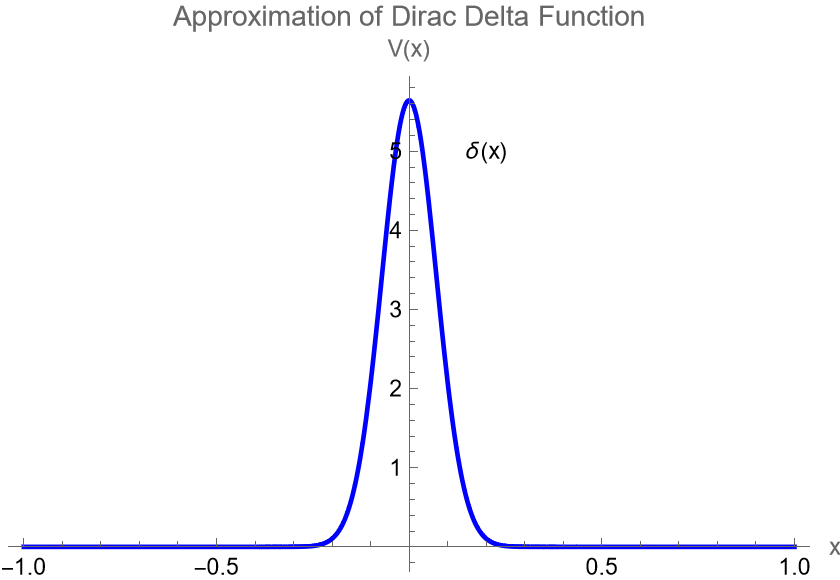
\includegraphics[width=0.4\textwidth]{figure/delta函数势.png}
        \caption{$\delta$函数势}
        \label{fig:delta函数势}
    \end{figure}
    \item 
    Consider double delta function potential
    \begin{equation*}
        V(x)=-\alpha\left(\delta(x+a)+\delta(x-a)\right)
    \end{equation*}
    where $\alpha$and $a$ are positive and real.
    
    \begin{enumerate}
        \item[(a)] Sketch the potential
        \item[(b)] Consider a plane wave travel from $-x-$axies to the $+x-$axies direction , find out the reflection rate and transition rate for theregions
        \item[(c)] How many bound state does it possess? Find out the allowed energies for$\ \displaystyle\alpha=\frac{\hbar^2}{4ma}$ and for$\ \displaystyle\alpha=\frac{\hbar^2}{ma}$ and sketch the wave function
    \end{enumerate}
\end{enumerate}


\begin{solution}
    \begin{enumerate}
        \item \[E\psi(x)=-\frac{\hbar^{2}}{2m}\frac{\partial^{2}\psi(x)}{\partial x^{2}}+\alpha\delta(x)\psi(x)\]
            从左边进行考虑,可得 
            \[\left\{\begin{array}{ll}\psi_1(x)=Ae^{ikx}+Be^{-ikx}&,x<0\\\psi_2(x)=Ce^{ikx}&,x>0\end{array}\right. \]
            在x=0 处波函数的连续性: 
            \[\psi(0^{-})=\psi(0^{+})\quad\Rightarrow\quad A+B=C \]
            在$x=0$ 处由于$\delta$函数势导致的波函数导数的不连续性: 
            \[\left.\frac{d\psi}{dx}\right|_{0^{+}}-\left.\frac{d\psi}{dx}\right|_{0^{-}}=\frac{2m\alpha}{\hbar^{2}}\psi(0)\]
            \[E\psi(x)=-\frac{\hbar^{2}}{2m}\frac{\partial^{2}\psi(x)}{\partial x^{2}}+\alpha\delta(x)\psi(x) \]
            从左边进行考虑,可得
            \[\left\{\begin{array}{ll}\psi_1(x)=Ae^{ikx}+Be^{-ikx}&,x<0\\\psi_2(x)=Ce^{ikx}&,x>0\end{array}\right. \]
            在x=0处波函数的连续性: 
            \[\psi(0^{-})=\psi(0^{+})\quad\Rightarrow\quad A+B=C \]
            在x=0处由于$\delta$函数势导致的波函数导数的不连续性: 
            \[\left.\frac{d\psi}{dx}\right|_{0^{+}}-\left.\frac{d\psi}{dx}\right|_{0^{-}}=\frac{2m\alpha}{\hbar^{2}}\psi(0)\]

            
                \begin{align*}
                    \left.\frac{d\psi}{dx}\right|_{0^-}&=ik(A-B) \\
                    \left.\frac{d\psi}{dx}\right|_{0^+}&=ikC \\
                    ikC-ik(A-B) &=\frac{2m\alpha}{\hbar^{2}}(A+B) \\
                    ik(C-A+B) &=\frac{2m\alpha}{\hbar^{2}}(A+B) \\
                    B&=\frac{m\alpha/\hbar^{2}}{ik-m\alpha/\hbar^{2}}A 
                \end{align*}
                求解可得
                \begin{align*}
                    B&=\frac{m\alpha/\hbar^{2}}{ik-m\alpha/\hbar^{2}}A \\
                    C&=\frac{ik}{ik-m\alpha/\hbar^{2}}A 
                \end{align*}
                
                于是可以求得,反射率和透射率为
                \begin{align*}
                    &R=\left|\frac{m\alpha/\hbar^{2}}{ik-m\alpha/\hbar^{2}}\right|^{2}=\frac{(m\alpha/\hbar^{2})^{2}}{k^{2}+(m\alpha/\hbar^{2})^{2}} \\
                &T=\left|\frac{ik}{ik-m\alpha/\hbar^{2}}\right|^{2}=\frac{k^{2}}{k^{2}+(m\alpha/\hbar^{2})^{2}} 
                \end{align*}
                
                很显然,有关系
                \[R+T=1\]
        \item 对于问题二,相对来说要复杂的多
        \begin{enumerate}
            \item[(a)]
            \begin{figure}[hbtp]
                \centering
                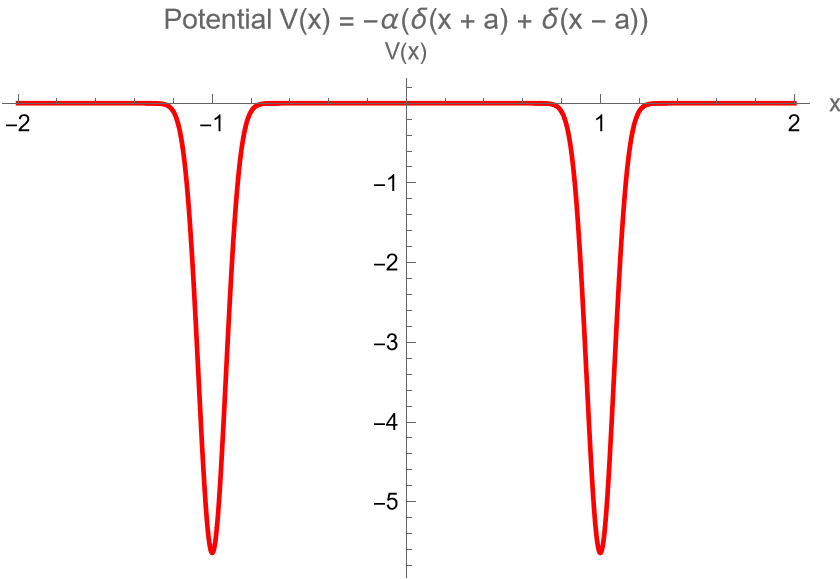
\includegraphics[width=0.4\textwidth]{figure/双delta函数势.png}
                \caption{$\delta$函数梳}
                \label{fig:delta函数梳}
            \end{figure}
            \item[(b)] 先给出在这个势函数下的波函数的方程
            \[
                \begin{cases}
                \psi_1\left(x\right)=Ae^{ikx}+Be^{-ikx},&-\infty<x<-a,\\
                \psi_2\left(x\right)=Ce^{ikx}+De^{-ikx},&-a<x<a,\\
                \psi_3\left(x\right)=Fe^{-ikx},&a<x<\infty.
                \end{cases}
            \]
            于是有
            \begin{align*}
                Ae^{-ika}+Be^{ika}&=Ce^{-ika}+De^{ika}\\
                Ce^{ika}+De^{-ika}&=Fe^{ika}\\
                (Ae^{-ika}-Be^{ika})-(Ce^{-ika}-De^{ika})&=\frac{2m\alpha}{ik\hbar^2}\left(Ce^{-ika}+De^{ika}\right)\\
                (Ce^{ika}-De^{-ika})-Fe^{ika}&=\frac{2m\alpha}{ik\hbar^2}Fe^{ika}
            \end{align*}

            
                令 $\beta=\frac{2m\alpha}{k\hbar^{2}}$ 
                \begin{align*}
                    \begin{pmatrix}
                        A\\B
                    \end{pmatrix}
                    &=\pmtwo{1+\frac{\beta}{2}}{\frac{\beta}{2}e^{i2ka}}{-\frac{\beta}{2}e^{-i2ka}}{1-\frac{\beta}{2}}
                    \begin{pmatrix}
                        C\\D
                    \end{pmatrix}\\
                    \begin{pmatrix}
                        C\\D
                    \end{pmatrix}
                    &=\pmtwo{1+\frac{\beta}{2}}{0}{-\frac{\beta}{2}e^{i2ka}}{0}
                    \begin{pmatrix}
                        F\\0
                    \end{pmatrix}\\
                \end{align*}
                
                因此,可以有
                \begin{align*}
                    \begin{pmatrix}
                        A\\B
                    \end{pmatrix}
                    &=\pmtwo{1+\frac{\beta}{2}}{\frac{\beta}{2}e^{i2ka}}{-\frac{\beta}{2}e^{-i2ka}}{1-\frac{\beta}{2}}
                    \begin{pmatrix}
                        \left(1+\frac{\beta}{2}\right)F\\-\frac{\beta}{2}e^{i2ka}F
                    \end{pmatrix}
                \end{align*}
                于是在$-\infty<x< -a$时, 
                \begin{align*}
                    |\frac{B}{A}|^{2}=R_{1}=\frac{\beta^2\left[(1+\frac{\beta}{2})^2+(1-\frac{\beta}{2})^2+2(1-\frac{\beta}{2})(1+\frac{\beta}{2}) cos(3ka)\right]}{4\left[\left(1+\frac{\beta}{2}\right)^4-\left(\frac{\beta}{4}\right)^4-2\left(1+\frac{\beta}{2}\right)^2\left(\frac{\beta}{4}\right)^2cos(4ka)\right]}
                \end{align*}
                
                于是在$-a<x<a$ 时
                \begin{align*}
                    T_{1}&=\left|\frac{C}{A}\right|^2=\frac{\left(\frac{\beta}{2}+1\right)^2}{\left(1+\frac{\beta}{2}\right)^4-\left(\frac{\beta}{4}\right)^4-2\left(1+\frac{\beta}{2}\right)^2\left(\frac{\beta}{4}\right)^2cos(4ka)} \\
                    R_{2}&=\left|\frac{D}{C}\right|^{2}=\frac{\beta^{2}}{4\left(\frac{\beta}{2}+1\right)^{2}} \\
                \end{align*}
                于是在 $a<x<\infty$时
                \begin{align*}
                    T_{2}=\left|\frac{E}{C}\right|^{2}=\frac{1}{\left(\frac{\beta}{2}+1\right)^{2}}
                \end{align*}
                
                此时,我们令
                \[g=\frac{1}{\beta}=\frac{\hbar^{2}k}{2m\alpha},\quad\psi=4ka \]
                则有
                \[ T_{\mathrm{总}}=\left|\frac{A}{E}\right|^{2}=\frac{8g^{4}}{8g^{4}+4g^{2}+1+(4g^{2}-1)\cos\varphi-4g\sin\varphi} \]
            
            \item[(c)] 比较显然的一件事是,波函数应当在无穷远处是趋近于0的,这也要求了波函数应该是一个在无穷远处是有限的,于是,我们可以得到波函数的形式为
            \[
                \begin{cases}
                \psi_1\left(x\right)=Ae^{ikx},&-\infty<x<-a,\\
                \psi_2\left(x\right)=Ce^{ikx}+De^{-ikx},&-a<x<a,\\
                \psi_3\left(x\right)=Fe^{-ikx},&a<x<\infty.
                \end{cases}
            \]
            其中,$k=\frac{-2mE}{\hbar^{2}}$
            由类似的边界条件,我们可以得到这样的线性方程组
            \begin{align*}
                kAe^{-ka}-k\left(Be^{-ka}-Ce^{ka}\right)&=\frac{2m\alpha}{\hbar^{2}}Ae^{-ka} \\
                kDe^{-ka}+k\left(Be^{ka}-Ce^{-ka}\right)&=\frac{2m\alpha}{\hbar^{2}}De^{-ka} \\
                Ae^{-ka}&=Be^{-ka}+Ce^{ka} \\
                De^{-ka}&=Be^{ka}+Ce^{-ka} 
            \end{align*}
            通过求解,我们知道
            \begin{align*}
                B&=(1-\frac{\beta}{2})A\\
                C&=\frac{\beta}{2}e^{-2ka}A\\
                D&=(1-\frac{\beta}{2})A+\frac{\beta}{2}e^{-2ka}A
            \end{align*}
            \begin{enumerate}
                \item[$\alpha=\frac{\hbar^2}{ma}$] 此时我们可以知道$A=D$,$\displaystyle B=C=\frac{}{}$
                \item[$\alpha=\frac{\hbar^2}{4m\alpha}$] 
            \end{enumerate}
        \end{enumerate}
    \end{enumerate}
\end{solution}







\section{三维定态薛定谔方程}
\subsection{三维定态薛定谔方程小计算20241107}
\begin{enumerate}
    \item Try to work out the energy spectrum and wave functions till $n=3$
    \item Check the Hydrogen spectral series numerically and the values we obtained from formula. Are they consistent? Why not?
\end{enumerate}


\begin{solution}
    正如我们所知道的,对于能级为$n$的能量以及波函数,我们有如下的公式:
    
    能谱:
    \begin{equation*}
        E_n=-\left[\frac{m}{2\hbar^2}\left(\frac{e^2}{4\pi\varepsilon_0}\right)^2\right]\frac{1}{n^2},\quad\quad n=1,2,3,...
    \end{equation*}
    
    波函数:
    \begin{equation*}
        \psi_{nlm}=\sqrt{\left(\frac{2}{na_0}\right)^3\frac{(n-l-1)!}{2n[(n+l)!]^3}}e^{-\frac{r}{na_0}}\left(\frac{2r}{na_0}\right)^l[L^{2l+1}_{n-l-1}\left(\frac{2r}{na_0}\right)]Y^{m}_{l}(\theta,\phi)
    \end{equation*}
    \begin{enumerate}
        \item 接下来我们来求解一下$n=1,2,3$的情况下的能量和波函数,由于$n=3$时会使得轨道角量子数$l=2,1,0$,而他们有分别对应着很多个磁量子数$m_{l=0}=0,m_{l=1}=1,0,-1,m_{l=2}=2,1,0,-1,-2$
        \begin{enumerate}
            \item[n=1时] 此时的能量为
            \begin{align*}
                E_1&=-\left[\frac{m}{2\hbar^2}\left(\frac{e^2}{4\pi\varepsilon_0}\right)^2\right]\\
                &=-13.6 eV
            \end{align*}

            而此时的轨道角量子数$l=0$,磁量子数为$m=0$,即
            \[ 
                \psi_{100} = \sqrt{\frac{2}{\pi a_0^3}} e^{-\frac{r}{a_0}} 
            \]
            \item[n=2时] 此时的能量为
            \begin{align*}
                E_2&=-\left[\frac{m}{2\hbar^2}\left(\frac{e^2}{4\pi\varepsilon_0}\right)^2\right]\frac{1}{2^2}\\
                &=-3.4 eV
            \end{align*}

            接下来看一看他的波函数有几种情况,由于$n=2$,因此$l=0,1$
            \begin{enumerate}
                \item[n=2,l=0时] 波函数的磁量子数为$m=0$
                \[ 
                    \psi_{200} = \sqrt{\frac{1}{8\pi a_0^3}} \left(2 - \frac{r}{a_0}\right) e^{-\frac{r}{2a_0}} 
                \]
                \item[n=2,l=1时] 波函数的磁量子数有三个$m=-1,0,1$ 
                \begin{enumerate}
                    \item[n=2,l=1,m=-1时] 波函数可以写为
                    \begin{align*}
                        \psi_{21-1} = \sqrt{\frac{1}{64\pi a_0^5}} r \sin{\theta} e^{-i\phi} e^{-\frac{r}{2a_0}}
                    \end{align*}
                    \item[n=2,l=1,m=0时] 波函数可以写为
                    \begin{align*}
                        \psi_{210} = \sqrt{\frac{1}{32\pi a_0^5}} r \cos{\theta} e^{-\frac{r}{2a_0}}
                    \end{align*}
                    \item[n=2,l=1,m=1时] 波函数可以写为 
                    \begin{align*}
                        \psi_{211} = -\sqrt{\frac{1}{64\pi a_0^5}} r \sin{\theta} e^{i\phi} e^{-\frac{r}{2a_0}}
                    \end{align*}
                \end{enumerate}
            \end{enumerate}
            \item[n=3时] 此时的能量为
            \begin{align*}
                E_3&=-\left[\frac{m}{2\hbar^2}\left(\frac{e^2}{4\pi\varepsilon_0}\right)^2\right]\frac{1}{3^2}\\
                &=-1.511 eV
            \end{align*}
            
            对于$n=3$的情况,就有三种轨道角量子数$l=0,1,2$,磁量子数$m$在底下分类讨论
            \begin{enumerate}
                \item[n=3,l=0时] 此时的磁量子数为$m=0$,因此波函数可以写为
                \begin{align*}
                    \psi_{300} = \sqrt{\frac{1}{108\pi a_0^3}} \left(27 - 18 \frac{r}{a_0} + 2 \left(\frac{r}{a_0}\right)^2\right) e^{-\frac{r}{3a_0}}
                \end{align*}
                \item[n=3,l=1时] 此时的磁量子数将值得被讨论,有$m=1,0,-1$
                \begin{enumerate}
                    \item[n=3,l=1,m=1时] 此时的波函数为
                    \begin{align*}
                        \psi_{311} = -\sqrt{\frac{1}{216\pi a_0^5}} \left(6r - r^2\right) \sin{\theta} e^{i\phi} e^{-\frac{r}{3a_0}}
                    \end{align*}
                    \item[n=3,l=1,m=0时] 此时的波函数为
                    \begin{align*}
                        \psi_{310} = \sqrt{\frac{1}{108\pi a_0^5}} \left(6r - r^2\right) \cos{\theta} e^{-\frac{r}{3a_0}}
                    \end{align*}
                    \item[n=3,l=1,m=-1时] 此时的波函数为
                    \begin{align*}
                        \psi_{31-1} = \sqrt{\frac{1}{216\pi a_0^5}} \left(6r - r^2\right) \sin{\theta} e^{-i\phi} e^{-\frac{r}{3a_0}}
                    \end{align*}
                \end{enumerate}
                \item[n=3,l=2时] 这个情况下的波函数就更多了,因为磁量子数$m=-2,-1,0,1,2$
                \begin{enumerate}
                    \item[n=3,l=2,m=-2时]
                    \begin{align*}
                        \psi_{32-2} = \sqrt{\frac{15}{2592\pi a_0^7}} r^2 \sin^2{\theta} e^{-2i\phi} e^{-\frac{r}{3a_0}}
                    \end{align*}
                    \item[n=3,l=2,m=-1时]
                    \begin{align*}
                        \psi_{32-1} = \sqrt{\frac{15}{648\pi a_0^7}} r^2 \sin{\theta} \cos{\theta} e^{-i\phi} e^{-\frac{r}{3a_0}}
                    \end{align*}
                    \item[n=3,l=2,m=0时]
                    \begin{align*}
                        \psi_{320} = \sqrt{\frac{5}{1296\pi a_0^7}} r^2 (3\cos^2{\theta} - 1) e^{-\frac{r}{3a_0}}
                    \end{align*}
                    \item[n=3,l=2,m=1时]
                    \begin{align*}
                        \psi_{321} = -\sqrt{\frac{15}{648\pi a_0^7}} r^2 \sin{\theta} \cos{\theta} e^{i\phi} e^{-\frac{r}{3a_0}} 
                    \end{align*}
                    \item[n=3,l=2,m=2时]
                    \begin{align*}
                        \psi_{322} = \sqrt{\frac{15}{2592\pi a_0^7}} r^2 \sin^2{\theta} e^{2i\phi} e^{-\frac{r}{3a_0}} 
                    \end{align*}
                \end{enumerate} 
            \end{enumerate}
        \end{enumerate}
    \end{enumerate}
\end{solution}






\subsection{坐标、动量、角动量对易关系证明20241107}
\begin{enumerate}
    \item Please verify
    \begin{enumerate}
        \item $[x,L_z]=-i\hbar y$
        \item $[y,L_z]=i\hbar x$
        \item $[p_x,L_z]=-i\hbar p_y$
        \item $[p_y,L_z]=i\hbar p_x$
    \end{enumerate}
\end{enumerate}

\begin{solution}
    \begin{enumerate}
        \item[(a)] 
        \begin{align*}
            [x,L_z]&=[x,xp_y-yp_x]\\
            &=[x,xp_y]-[x,yp_x]\\
            &=[x,x]p_y+x[x,p_y]-[x,y]p_x-y[x,p_x]\\
            &=0+0-0-i\hbar y\\
            &=-i\hbar y
        \end{align*}
        \item[(b)]
        \begin{align*}
            [y,L_z]&=[y,xp_y-yp_x]\\
            &=[y,xp_y]-[y,yp_x]\\
            &=[y,x]p_y+x[y,p_y]-[y,y]p_x+y[y,p_x]\\
            &=0+i\hbar x+0+0\\
            &=i\hbar x
        \end{align*}
        \item[(c)]
        \begin{align*}
            [p_x,L_z]&=[p_x,xp_y-yp_x]\\
            &=[p_x,xp_y]-[p_x,yp_x]\\
            &=[p_x,x]p_y+x[p_x,p_y]-[p_x,y]p_x-y[p_x,p_x]\\
            &=-i\hbar p_y+0-0-0\\
            &=-i\hbar p_y
        \end{align*}
        \item[(d)]
        \begin{align*}
            [p_y,L_z]&=[p_y,xp_y-yp_x]\\
            &=[p_y,xp_y]-[p_y,yp_x]\\
            &=[p_y,x]p_y+x[p_y,p_y]-[p_y,y]p_x+y[p_y,p_x]\\
            &=0+0+i\hbar p_x+0\\
            &=i\hbar p_x
        \end{align*}
    \end{enumerate}
\end{solution}







\subsection{角动量的对易关系计算20241108}
\begin{enumerate}
    \item Please verify
    \begin{enumerate}
        \item $[L_i,x_j]=\epsilon_{ijk}x_k$
        \item $[L_i,p_j]=\epsilon_{ijk}p_k$
    \end{enumerate}
    \item Please verify
    \begin{enumerate}
        \item $[L_i,L_j]=i\hbar\epsilon_{ijk} L_k$
    \end{enumerate}
\end{enumerate}

\begin{solution}
    \begin{enumerate}
        \item
        \begin{enumerate}
            \item[(a)] 
            \begin{align*}
                [L_i,x_j]&=\epsilon_{inm}[x_np_m,x_j]\\
                &=\epsilon_{inm}\left(x_n[p_m,x_j]+[x_n,x_j]p_m\right)\\
                &=-\epsilon_{inm}x_ni\hbar\delta_{mj}\\
                &=-\epsilon_{inj}x_n\\
                &=\epsilon_{ijn}x_n
            \end{align*}
            \item[(b)] 
            \begin{align*}
                [L_i,p_j]&=\epsilon_{inm}[x_np_m,p_j]\\
                &=\epsilon_{inm}\left(x_n[p_m,p_j]+[x_n,p_j]p_m\right)\\
                &=\epsilon_{inm}i\hbar \delta_{nj}p_m\\
                &=\epsilon_{ijm}p_m
            \end{align*}
        \end{enumerate}
        \item 
        \begin{align*}
            [L_i,L_j]&=[\epsilon_{inm}x_np_m,\epsilon_{jlr}x_lp_r]\\
            &=\epsilon_{inm}\epsilon_{jlr}[x_np_m,x_lp_p]\\
            &=\epsilon_{inm}\epsilon_{jlr}\{x_n[p_m,x_lp_r]+[x_n,x_lp_r]p_m\}\\
            &=\epsilon_{inm}\epsilon_{jlr}\{x_nx_l[p_m,p_r]+x_n[p_m,x_l]p_r+x_l[x_n,p_r]p_m+[x_n,x_l]p_rp_m\}\\
            &=\epsilon_{inm}\epsilon_{jlr}\left(-i\hbar x_np_r\delta_{lm}+i\hbar x_lp_m\delta_{nr}\right)\\
            &=i\hbar\epsilon_{inm}\epsilon_{jln}x_lp_m-i\hbar\epsilon_{inm}\epsilon_{jmr}x_np_r\\
            &=(\delta_{mj}\delta_{il}-\delta_{ml}\delta{ij})i\hbar x_lp_m+(\delta_{ir}\delta_{nj}-\delta_{ij}\delta_{rn})(-i\hbar x_np_r)\\
            &=i\hbar x_ip_j-i\hbar x_mp_m\delta_{ij}-i\hbar x_ip_i+i\hbar x_np_n\delta_{ij}\\
            &=i\hbar(x_ip_j-x_jp_i)\\
            &=i\hbar\epsilon_{kij}L_k
        \end{align*}
    \end{enumerate}
\end{solution}




\subsection{Pauli Matrix的计算20241118}

The Pauli Matrix is defined as 
\begin{align*}
    \sigma_1=\pmtwo{0}{1}{1}{0},\sigma_2=\pmtwo{0}{-i}{i}{0},\sigma_3=\pmtwo{1}{0}{0}{-1}
\end{align*}

Please proof that
\begin{enumerate}
    \item[(1)] \[[\sigma_i,\sigma_j]=2i\epsilon_{ijk}\sigma_k\]
    \item[(2)] \[\{\sigma_i,\sigma_j\}=\sigma_i\sigma_j+\sigma_j\sigma_i=2\delta_{ij}I\] where $\{A,B\} $ is anti-commutation relation. 
    \item[(3)] \[\sigma_i\sigma_j=\delta_{ij}I+i\epsilon_{ijk}\sigma_k\]
    \item[(4)] By define 
    \[\vec{A}\cdot\vec{\sigma}=(A_ie_i)(\sigma_je_j)=A_i\sigma_j\delta_{ij}=A_i\sigma_i\]

    show that
    \[(\vec{A}\cdot\vec{\sigma})(\vec{B}\cdot\vec{\sigma})=(\vec{A}\cdot \vec{B})I+i(\vec{A}\times \vec{B})\vec{\sigma}\]
    \item[(5)] \[\frac{\vec{\sigma}}{2}\times \frac{\vec{\sigma}}{2}=i\frac{\vec{\sigma}}{2}\]
    \item[(6)] By define
    \[\vec{A}=A\vec{n}\]
    show that
    \[e^{iA(\vec{n}\cdot\vec{\sigma})}=I\cos{A}+i(\vec{n}\cdot\vec{\sigma})\sin{A}\]
\end{enumerate}


\begin{solution}
    \ \\
    \begin{enumerate}
        \item[(1)] 事实上,这个结论很trivial,我们知道泡利矩阵与$SU(2)$的李代数是同构的,而$SU(2)$是$SO(3)$的双覆盖群,所以泡利矩阵也间接的与$SO(3)$的李代数同构,也就是说和自旋的性质是相同的,而我们还可以知道,自旋算符可以表示为泡利矩阵的线性组合
        \begin{align*}
            S_i=\frac{\hbar}{2}\sigma_i
        \end{align*}
        而我们知道自旋算符的对易关系为
        \begin{align*}
            [S_i,S_j]=i\epsilon_{ijk}S_k
        \end{align*}
        于是也有
        \begin{align*}
            [\sigma_i,\sigma_j]=2i\epsilon_{ijk}\sigma_k
        \end{align*}
        \item[(2)] 这一题老老实实的计算一下
        
        首先是$\{\sigma_1,\sigma_2\}$
        \begin{align*}
            \{\sigma_1,\sigma_2\}&=\sigma_1\sigma_2+\sigma_2\sigma_1\\
            &=\pmtwo{0}{1}{1}{0}\pmtwo{0}{-i}{i}{0}+\pmtwo{0}{-i}{i}{0}\pmtwo{0}{1}{1}{0}\\
            &=\pmtwo{i}{0}{0}{-i}+\pmtwo{-i}{0}{0}{i}\\
            &=\pmtwo{0}{0}{0}{0}
        \end{align*}

        接下来是$\{\sigma_2,\sigma_3\}$
        \begin{align*}
            \{\sigma_2,\sigma_3\}&=\sigma_2\sigma_3+\sigma_3\sigma_2\\
            &=\pmtwo{0}{-i}{i}{0}\pmtwo{1}{0}{0}{-1}+\pmtwo{1}{0}{0}{-1}\pmtwo{0}{-i}{i}{0}\\
            &=\pmtwo{0}{i}{i}{0}+\pmtwo{0}{-i}{-i}{0}\\
            &=\pmtwo{0}{0}{0}{0}
        \end{align*}

        然后是$\{\sigma_3,\sigma_1\}$
        \begin{align*}
            \{\sigma_3,\sigma_1\}&=\sigma_1\sigma_3+\sigma_3\sigma_1\\
            &=\pmtwo{0}{1}{1}{0}\pmtwo{1}{0}{0}{-1}+\pmtwo{1}{0}{0}{-1}\pmtwo{0}{1}{1}{0}\\
            &=\pmtwo{0}{-1}{1}{0}+\pmtwo{0}{1}{-1}{0}\\
            &=\pmtwo{0}{0}{0}{0}
        \end{align*}
        
        最后是$\{\sigma_1,\sigma_1\}$
        \begin{align*}
            \{\sigma_1,\sigma_1\}&=2\sigma_1\sigma_1\\
            &=2\pmtwo{0}{1}{1}{0}\pmtwo{0}{1}{1}{0}\\
            &=2\pmtwo{1}{0}{0}{1}\\
            &=2I
        \end{align*}
        
        综合以上所计算得到的,我们可以得出一个归纳性结论
        \begin{align*}
            \{\sigma_i,\sigma_j\}=2\delta_{ij}I
        \end{align*}
        \item[(3)] 综合第$(1)$问和第$(2)$问,我们已经知道了$[\sigma_i,\sigma_j]$与$\{\sigma_i,\sigma_j\}$,因此,可以得出
        \begin{align*}
            [\sigma_i,\sigma_j]+\{\sigma_i,\sigma_j\}&=(\sigma_i\sigma_j-\sigma_j\sigma_i)+(\sigma_i\sigma_j+\sigma_j\sigma_i)\\
            &=2\sigma_i\sigma_j\\
            &=2i\epsilon_{ijk}\sigma_k+2\delta_{ij}I
        \end{align*}

        于是,我们得到了最终需要证明的表达式
        \begin{align*}
            \sigma_i\sigma_j&=i\epsilon_{ijk}\sigma_k+\delta_{ij}I
        \end{align*}
        \item[(4)] 
        这一题在一开始给我们定义了Pauli矩阵与矢量的内积,我们可以直接利用这个定义来计算
        \begin{align*}
            (\vec{A}\cdot\vec{\sigma})(\vec{B}\cdot\vec{\sigma})&=(A_i\sigma_i)(B_j\sigma_j)\\
            &=A_iB_j(\sigma_i\sigma_j)\\
            &=A_iB_j(\delta_{ij}I+i\epsilon_{ijk}\sigma_k)\\
            &=(\delta_{ij}A_iB_j)I+(\varepsilon_{ijk}A_iB_j\sigma_k)\\
            &=(\vec{A}\cdot\vec{B})I+i(\vec{A}\times\vec{B})\vec{\sigma}
        \end{align*}
        \item[(5)] 直接开始计算吧
        \begin{align*}
            \frac{\vec{\sigma}}{2}\times\frac{\vec{\sigma}}{2}&=\frac{1}{4}(\vec{\sigma}\times\vec{\sigma})\\
            &=\frac{1}{4}\vmthree{i}{j}{k}{\sigma_1}{\sigma_2}{\sigma_3}{\sigma_1}{\sigma_2}{\sigma_3}\\
            &=\frac{1}{4}\epsilon_{ijk}\sigma_i\sigma_j\\
            &=\frac{1}{4}\epsilon_{ijk}\left(\epsilon_{ijl}\sigma_l+\delta_{ij}I\right)\\
            &=\frac{1}{4}\left(\epsilon_{ijk}\epsilon_{ijl}\sigma_l+\epsilon_{ijk}\delta_{ij}I\right)\\
            &=\frac{1}{4}\left(\delta_{kl}\sigma_l+0\right)\\
            &=\frac{1}{4}\sigma_k
        \end{align*}
    \end{enumerate}
\end{solution}
\newpage
\section{量子多体系统}
\subsection{三粒子系统的一维无限位能阱问题20241125}
Consider a 1-D infinite square wall which contains 3 particles.Please write down the wave function of ground state and the first excited state.
\begin{enumerate}
    \item Three distinguishable particles
    \item Two identical bosons and one fermion
    \item one bosons and Two identical fermion
    \item Three identical bosons
    \item Three identical fermions
\end{enumerate}

\section{微扰法}
\subsection{微扰法20241212}
Using perturbation method for the 2D infinite wall:
\begin{align*}
    V(x,y)=
    \begin{cases}
        V,&\frac{L}{2}\leq x \leq L,0\leq y\leq L\\
        0,&otherwise\\
        \infty,&x<0||x>L,y<0||y>L
    \end{cases}
\end{align*}
\begin{enumerate}
    \item  Find out the spectrum and wave function without perturbation.
    \item Find out the first order correction of ground state and the first excited state for wave function and energy spectrum.
\end{enumerate}

\begin{solution}
    本题是一个二维空间中的薛定谔方程,首先给出我们的定态薛定谔方程
    \begin{align*}
        \frac{\hbar^2}{2m}\nabla^2\psi+(E-V)\psi=0
    \end{align*}

    \begin{enumerate}
        \item 首先是求解没有微扰的情况,此时的$V(x,y)=0(0\leq x \leq L,0\leq y\leq L)$
        
        这时的薛定谔方程为
        \begin{align*}
            \frac{\hbar^2}{2m}\nabla^2\psi+E\psi&=0
        \end{align*}

        将波函数分解为
        \[
            \psi(x,y)=\psi_x(x)\psi_y(y)
        \]

        因此问我我们可以分别求解$\psi_x(x)$和$\psi_y(y)$的方程,而在这道题当中,很显然,$\psi_x(x)$与$\psi_y(y)$的形式是一致的,因此我们只需要求解一个方程即可,而这个方程就是一维无限深势阱的方程,于是,直接拿出答案吧
        \begin{align*}
            \psi_{xn}(x)&=\sqrt{\frac{2}{L}}\sin(\frac{n\pi}{L}x)\\
            E_{xn}&=\frac{\pi^2n_x^2\hbar^2}{2mL^2}
        \end{align*}

        于是我们可以有
        \begin{align*}
            \psi_{n_xn_y}(x,y)&=\frac{2}{L}\sin(\frac{n_x\pi}{L}x)\sin(\frac{n_y\pi}{L}y)\\
            E_{n_xn_y}&=\frac{\pi^2\hbar^2}{2mL^2}(n_x^2+n_y^2)
        \end{align*}
        \item 这道题给定了我们微扰,要求我们找到基态和第一级激发态的波函数与能谱的一阶修正
    \end{enumerate}
\end{solution}






\section{变分原理}
\subsection{变分原理20241212}
Consider 2D infinite wall 
\begin{align*}
    V(x,y)=
    \begin{cases}
        0,&0\leq x \leq L,0\leq y\leq L\\
        \infty,&otherwise    
    \end{cases}
\end{align*}

Try out an arbitrary wave function and find out the upper limit of ground state energy $E_g$.


\begin{solution}
    根据边界条件
    \[
        \psi(0,y)=\psi(L,y)=\psi(x,0)=\psi(x,L)
    \]

    于是,我们可以猜测波函数的形式为一个三角函数,即
    \begin{align*}
        \psi(x,y)=A\sin(\frac{\pi}{L}x)\sin(\frac{\pi}{L}y)
    \end{align*}

    利用归一化条件
    \begin{align*}
        \int_{0}^{L}\int_{0}^{L}|\psi(x,y)|^2dxdy&=1\\
        \Rightarrow A&=\frac{2}{L}
    \end{align*}

    有了这个猜测解,我们就可以去预估一下基态能量的上界
    \begin{align*}
        \expectation{H}&=\int_{0}^{L}\psi^*H\psi dxdy\\
        &=A^2\int_{0}^{L}\int_{0}^{L}\left(\sin(\frac{\pi}{L}x)\sin(\frac{\pi}{L}y)\right)\left(-\frac{\hbar^2}{2m}\right)\left(\sin(\frac{\pi}{L}x)\sin(\frac{\pi}{L}y)\right)dxdy\\
        &=\frac{4}{L^2}\frac{\pi^2}{L^2}\frac{\hbar^2}{2m}\cdot2\cdot\frac{\pi^2}{4}\\
        &=\frac{\pi^2\hbar^2}{mL^2}
    \end{align*}

    因此,根据该波函数所猜测出的基态能量上确界为$\dfrac{\pi^2\hbar^2}{mL^2}$
\end{solution}



\section{WKB 近似}
\subsection{WKB 近似20241216}
Consider 
\begin{align*}
    V(x)=
    \begin{cases}
        V,\quad 0\leq x\leq L\\
        0,\quad elsewhere
    \end{cases}
\end{align*}

By using WKB approximation,please try to analysis 
\begin{enumerate}
    \item E>V
    \item E<V
\end{enumerate}


\begin{solution}
    \begin{enumerate}
        \item 第一小问当中,需要分析的区域是$E>V$,这是经典力学所允许的区域,因此,我们直接代入到经典区域的WKB近似公式
        \begin{align*}
            \psi(x)\cong \frac{1}{\sqrt{p(x)}}\left[C_+e^{i\phi(x)}+C_-e^{-i\phi(x)}\right]
        \end{align*}

        其中
        \begin{align*}
            \psi(x)=\frac{1}{\hbar}\int_{0}^{x}p(x^\prime)dx^\prime
        \end{align*}

        
        
        将这个条件带入到我们的WKB近似公式当中
        \item 第二小问当中,需要分析的区域是$E<V$,这是经典力学所禁止的区域,也就是所谓的“隧穿”效应
        
        考虑到这是一个一维有限方势垒,因此我们知道其将会有一个透射波,一个入射波和一个反射波,而入射波与反射波是存在于$x<0$的区域,而透射波则是存在于$x>0$的区域,在这样的区域当中势能为0,即$V=0$,此时我们会有
        \begin{align*}
            \psi_1(x)&=Ae^{ikx}+Be^{-ikx},x<0\\
            \psi_3(x)&=Fe^{ikx},x>L
        \end{align*}

        而对于中间部分,我们可以用WKB近似为
        \begin{align*}
            \psi_2(x)=\frac{C}{\sqrt{|p(x)|}}e^{\displaystyle\frac{1}{\hbar}\int_{0}^{x}|p(x)|dt}+\frac{D}{\sqrt{|p(x)|}}e^{\displaystyle-\frac{1}{\hbar}\int_{0}^{x}|p(x)|dt}
        \end{align*}

    根据这个式子,我们知道,当势垒足够宽的时候,此时的$C$将可以忽略不计,于是入射波与透射波的强度比将会近似的等于波函数在势垒当中的衰减程度,即
    \begin{align*}
        T=\frac{|F|}{|A|}&\cong  e^{\displaystyle\frac{1}{\hbar}\int_{0}^{L}|p(x)|dx}\\
        &= e^{\displaystyle\frac{2m(E-V)}{\hbar}L}
    \end{align*}
    \end{enumerate}
\end{solution}
























\newpage
\section{附录}










\end{document}